The amount of protein sequences in UniProtKB has been growing exponentially from 2008 to 2018,
as shown in (Fig. \ref{fig:uniprot_growth}).
As on the moment this paragraph was written,
UniprotKB contained a total of 181,252,700 protein sequences.
562,253 were reviewed and part of the UniProtKB/Swiss-Prot database, 
the remaining 180,690,447 unreviewed sequences part of the UniprotKB/TrEMBL database.
This suggest that the exponential growth is still going on.
Translated proteomes are available for over 84 thousand different species with completely sequenced genomes.
Curators may target specific taxa to fill gabs in the taxonomic space,
and individual users can request for additional proteome imports
(\cite{uniprot2019}).


~\begin{figure}[h!]
	~\begin{subfigure}[b]{\linewidth}
		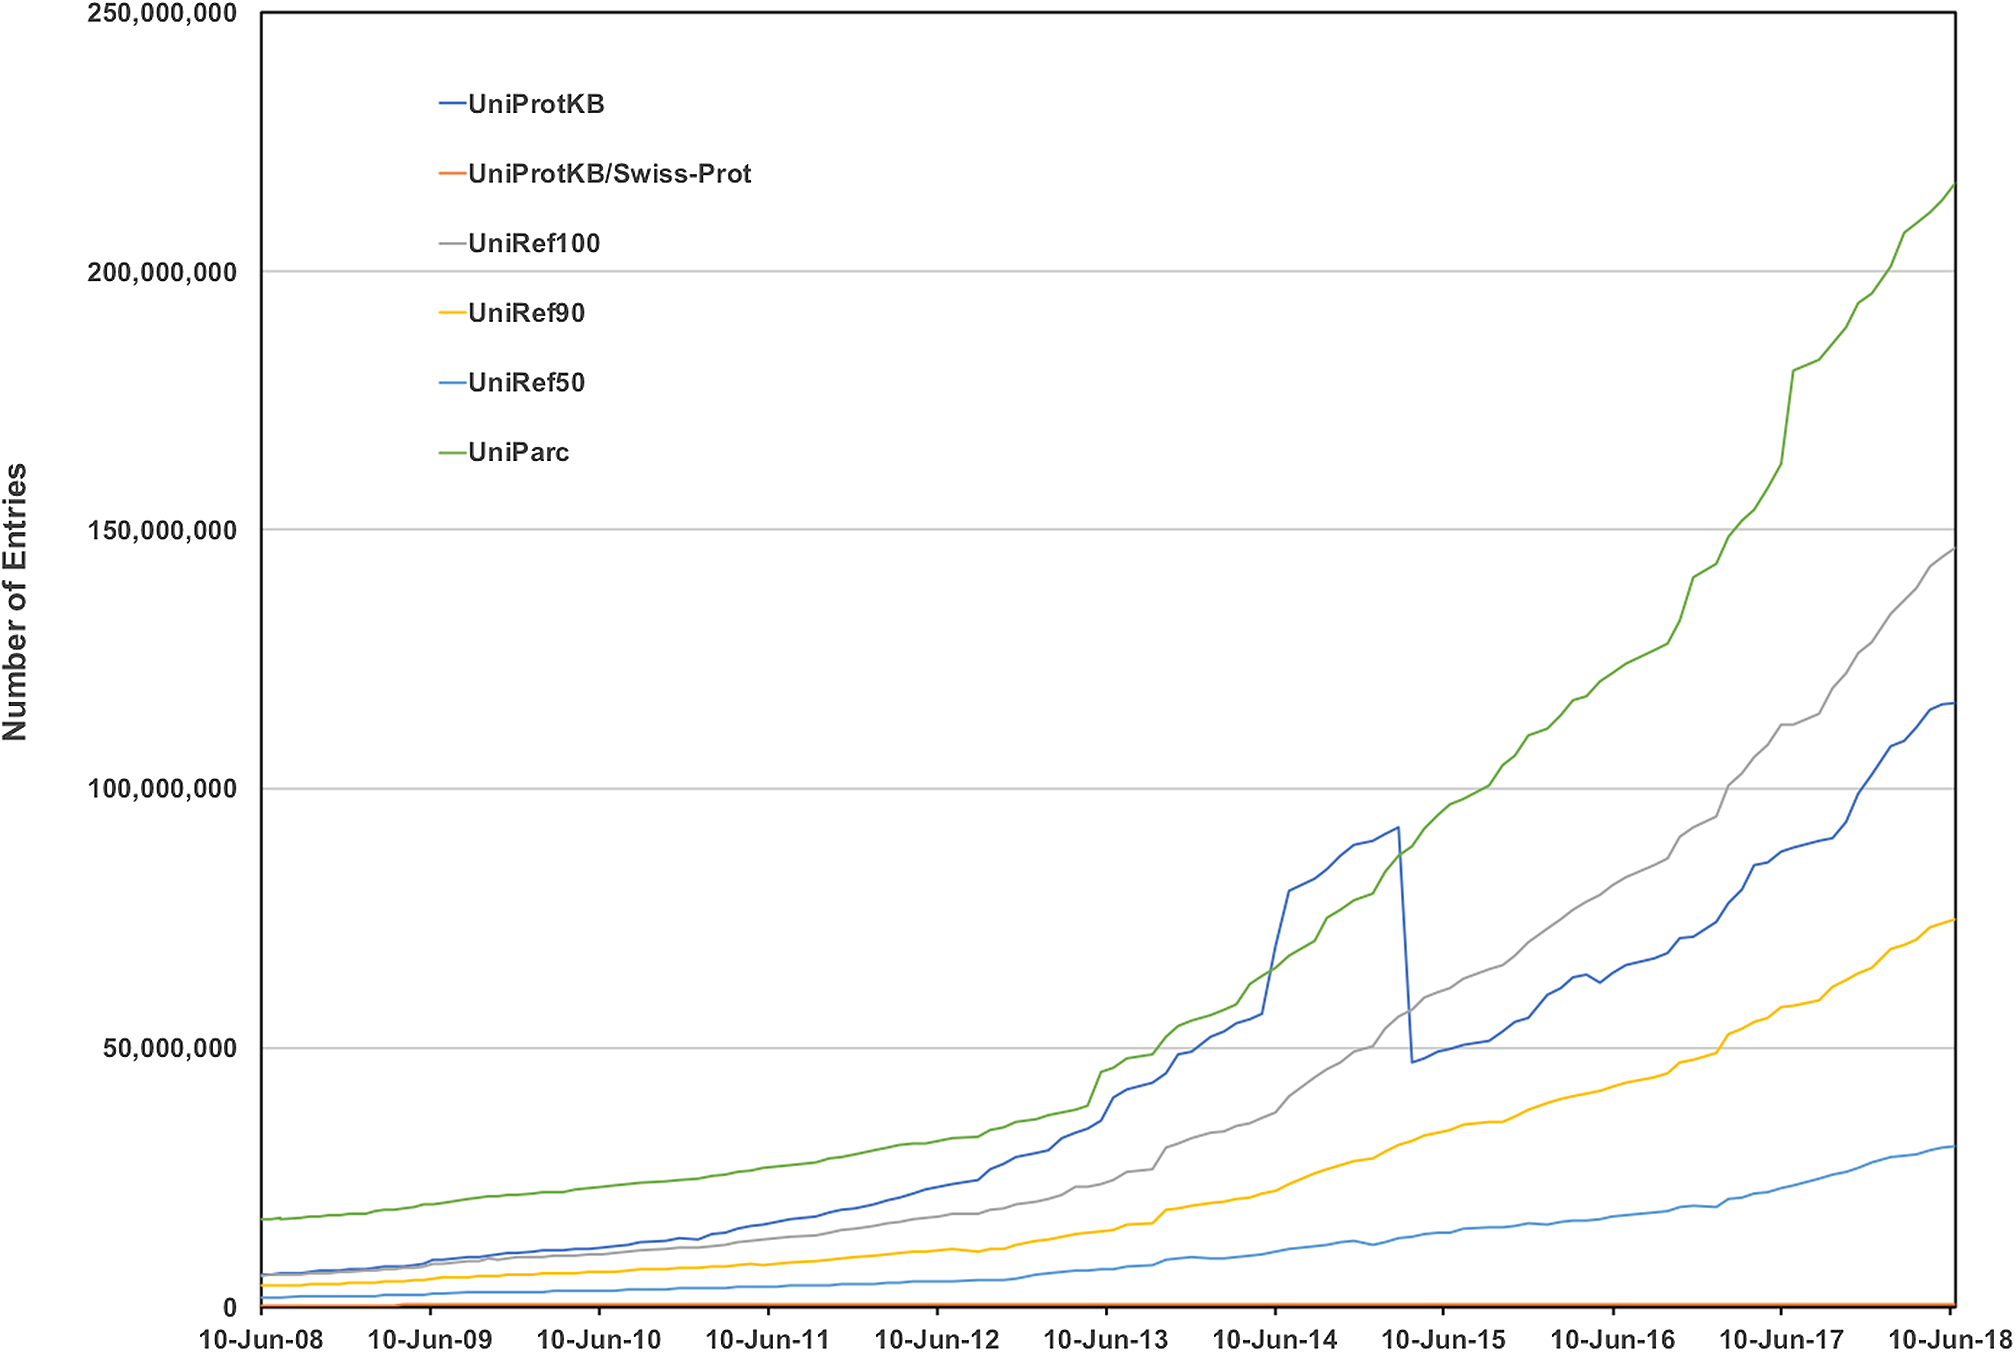
\includegraphics[width=\linewidth]
		{./literature_review/UniProtKB/database_growth/img/number_of_sequences.jpeg}
	~\end{subfigure}
	\caption{
		\textbf{Growth of UniProt sequences from 2008 to 2018.}	
		The graphs shows the growth curves of the different databases.
		Except for UniProtKB/Swiss-Prot, all databases display an overall exponential growth.
		The fall in the UniProtKB curve corresponds with a redundancy removal performed in 2015
		(from \cite{uniprot2019}).
		}
	\label{fig:uniprot_growth}
~\end{figure}

